\section{Алгоритмы генерации доменных имен}\label{dga}
Алгоритмы генерации доменных имен (DGA) представляют собой алгоритмы, используемые вредоносным программным обеспечением для генерации большого количества псевдослучайных доменных имен, которые позволят им установить соединение с управляющим командным центром. Тем самым они обеспечивают мощный слой защиты инфраструктуры ботнетов. С первого взгляда концепция создания большого количества доменных имен для установки связи кажется несложной, но методы, используемые для создания произвольных строк, часто скрываются за разными слоями обфускации. Это делается, в первую очередь, для усложнения процесса обратной разработки и получения модели функционирования того или иного семейства алгоритмов. В разделе \ref{work_princip} рассмотрены общие принципы алгоритмов генерации доменных имен, а раздел \ref{dga_teor} раскрывает особенности реализаций некоторых из рассмотренных алгоритмов.

    \subsection{Общие принципы работы}\label{work_princip}
        Общий принцип работы алгоритмов генерации доменных имен представлен на рис. \ref{dga_work}. В общем случае вредоносному файлу необходим какой-либо параметр для инициализации генератора псевдослучайных чисел (ГПСЧ). В качестве этого параметра может выступать любой параметр, который будет известен вредоносному файлу и владельцу ботнета. В нашем случае - это значение текущей даты и времени. Вредоносный файл, используя протокол HTTP посылает запрос на сайт cnn.com. В ответ на этот запрос, cnn.com возвращает в заголовках HTTP ответа текущие значения времени и даты в формате GMT. Владелец ботнета таким же способом получает текущие значения времени и даты в формате GMT. Далее, эти значения, попадают в сам алгоритм генерации доменных имен, инициализируя ГПСЧ, который может иметь вид, например, линейного конгруэнтного генератора или  регистра сдвига с обратной связью. Поэтому, используя одинаковые вектора инициализации, вредоносный файл и владелец ботнета получают идентичные таблицы доменных имен.
        После этого, владельцу ботнета достаточно зарегистрировать лишь один домен, для того, чтобы вредоносный файл, рекурсивно посылая запросы к DNS серверу, получил IP адрес управляющего сервера для дальнейшей установки с ним соединения и получения команд.
        \addimghere{images/dga_work}{0.8}{Общий принцип работы}{dga_work} %исправить картинку

    \subsection{Рассмотренные алгоритмы}\label{dga_teor}
    В ходе выполнения данной работы были проанализированы 8 разновидностей алгоритмов генерации доменных имен, а именно: Conficker, Cryptolocker, Ramdo, PushDo, Zeus, Tinba, Rovnix, Matsnu. Для каждого из них, путём обратной разработки, были составлены модели работы алгоритмов генерации доменных имен. Данные модели были реализованы на языках программирования высокого уровня. Далее в работе представлены описание и особенности работы каждого из этих алгоритмов.

Conficker - вирус, впервые появившийся в 2008 году, использующий для заражения машин популярную уязвимость MS08-067. Этот вирус одним из первых применил технику DGA. Процесс генерации доменного имени можно описать пятью шагами, как показано на рис. \ref{conficker_dga}, а его архитектура идентична принципу, описанному в разделе \ref{work_princip}.
\addimghere{images/conficker}{0.4}{Принцип работы conficker DGA}{conficker_dga}

Cryptolocker - имя вредоносных программ вида троян-вымогатель (ransomware). Целью данного вируса являются системы Microsoft Windows. Cryptolocker полностью шифрует содержимое файловой системы жертвы и требует выплаты денежной суммы для получения ключа дешифрования. Cryptolocker DGA относительно прост, однако использует множество приемов, которые осложняют процесс его обратной разработки. Его алгоритм использует для инициализации 4 значения - ключ, день, месяц, год.
Ключ может быть константой или рассчитываться по формуле \ref{crypto_key}.
\begin{equation}\label{crypto_key}
key = ((key * 0x10624DD3) >> 6) * 0xFFFFFC18)+ key
\end{equation}
В данной работе за значение ключа взята константа 0x41.
Каждый символ рассчитывается по формуле \ref{crypto_chr}.
\begin{equation}\label{crypto_chr}
chr(ord(a) + (year \; xor \; month\; xor \;date) \;\% \;25)
\end{equation}
А длина доменного имени составляет значение, рассчитанное по формуле \ref{crypto_lenght}.
\begin{equation}\label{crypto_lenght}
date>>3 \; xor \; year>>8 \; xor  \;year>>11 \; and \; 3 + 12
\end{equation}
В финальной стадии генерации доменного имени добавляется домен верхнего уровня, который последовательно выбирается из массива зашитых значений.

PushDo - ботнет, впервые появившийся в 2007 году. Для установки связи с командным сервером использует два механизма. Первый - зашитые доменные имена, и второй - DGA. Второй механизм имеет четыре составляющие, а именно: системное время, вектор инициализации, функцию хеширования MD5 и сам генератор доменных имен. Каждый день, при генерации первого доменного имени вектору инициализации присваивается значение системного времени, которое получается путем вызова WINAPI функции GetLocalTime, операций битового сдвига и XOR. После этого, вектор инициализации попадает на вход функции хеширования MD5, вывод которой, в свою очередь, попадает в генератор доменного имени и в вектор инициализации генерации следующего доменного имени. Однако, вектор инициализации следующего доменного имени берет не весь результат функции MD5, а лишь первые её 4 байта. Схема работы этого алгоритма генерации доменных имен представлена на рис. \ref{PushDo}.
\addimghere{images/PushDo}{0.8}{Принцип работы PushDo DGA}{PushDo}
Отдельно стоит рассмотреть генератор доменного имени, получающий на вход результат функции MD5. Каждый экземпляр такого генератора имеет четыре уникальных строки. Это позволяет обновлять генератор с каждой новой версией ботнета или иметь множество непересекающихся ботнетов одного и того же типа. Сначала генератор вычисляет длину доменного имени. Она рассчитывается делением первых четырех байт на 4 и лежит в пределах от 9 до 12. Далее, специальный цикл, используя остаток от деления, переводит вывод функции MD5 в читаемое доменное имя и добавляет к нему домен верхнего уровня. В итоге каждый день PushDo DGA генерирует 30 доменных имен, зависящих не только от системного времени, но и от зашитых значений - специальных строк генератора.

Zeus - семейство вредоносных программ, ворующих аутентификационноые данные, которое впервые появилось в 2007 году. Первые два варианта этого ботнета базировались на зашитых централизованных адресах управляющих серверов. Эти сервера постоянно отслеживались и отключались при помощи антивирусных компаний и центров реагирования на инциденты информационной безопасности. Именно поэтому, в 2011 году было обнаружено появление новой версии этого ботнета, который использует одноранговые сети и DGA для защиты своей инфраструктуры. В первую очередь, защита построена на одноранговых сетях, однако если все зараженные машины не отвечают, то используется DGA. Схема его реализация схожа с алгоритмом, используемым в ботнете PushDo. Алгоритм также использует системное время, алгоритм хеширования MD5 и генератор доменного имени. Однако, в отличие от PushDo, системное время является вектором инициализации для всех доменных имен, генерируемых каждую неделю, а номер доменного имени является параметром salt в функции хеширования MD5. Генератор доменного имени можно представить в виде следующего псевдокода.
\begin{lstlisting}
hash = MD5(time+salt)
name = ""
for (j = 0; j < len(hash); j++) {
    c1 = (hash[j] & 0x1F) + ’a’;
    c2 = (hash[j] / 8) + ’a’;
    if(c1 != c2 && c1 <= ’z’) name += c1;
    if(c1 != c2 && c2 <= ’z’) name += c2;
}
\end{lstlisting}
Листинг 1.1 - генератор доменного имени.

Семейство Ramdo, впервые обнаруженное в декабре 2013 года, кардинально отличается от других ботнетов. Ramdo использует множество приемов антиотладки, а также использует технологию double flux для установки соединения с управляющими серверами. Несмотря на сложность обратной разработки, данный ботнет имеет достаточно простой и небольшой DGA, который основывается на зашитой константе и итераторе, основанном на регистре сдвига и булевой операции исключающее или. Для формализации модели DGA данного семейства в работе использован исходный код из работы [15]. Кроме этого, идентичную модель DGA использует и ботнет Tinba, более известный как Tiny Banker. Основное отличие лишь в том, что для генерации следующего доменного имени Tinba использует также зашитый первоначальный адрес управляющего сервера.

Бурное развитие методов идентификации и фильтрации вредоносных доменных имен привело к развитию новых видов DGA. Примерами являются алгоритмы генерации доменных имен ботнетов Rovnix и Matsnu. Их алгоритмы проектировались специально для обхода систем идентификации, построенных на количественной оценки энтропии доменного имени или лингвистических моделях, например N-gram. Rovnix первым из ботнетов начал использовать специально заготовленный текст для генерации доменного имени. В качестве такого текста Rovnix использует декларацию о независимости США. На основе системного времени Rovnix выбирает слова из данного текста и конкатенирует их до достижения определенной длины. Ботнет Matsnu имеет схожий подход, вредоносная программа использует два зашитых словаря, один из которых содержит существительные, а второй глаголы. Тем самым, основываясь на системном времени, алгоритм генерации доменного имени выбирает существительное, а затем выбирает глаголы до достижения необходимой длины доменного имени. Стоит отметить, что подходы этих двух ботнетов действительно с легкостью обходят системы распознавания, основанные лишь на энтропийной оценке, поэтому для идентификации этих классов вредоносных доменных имен требуются более сложные модели, описанные в главах \ref{be_class_exp} и \ref{lstm_class_exp}.
\clearpage

\section{Существующие подходы к классификации}\label{be_class}
В настоящее время существует множество работ, связанных с анализом алгоритмов генерации доменных имен. Проблемы автоматического анализа алгоритмов DGA и пути их решения можно найти в статье [1]. Большие объемы данных, которые можно получить путем мониторинга сетевой активности ботнетов или путем обратной разработки алгоритмов генерации доменных имен, позволяют иcпользовать методы машинного обучения. Идея их применения освещена в работе [7]. Так, ряд известных компаний, занимающихся информационной безопасностью (Damballa, OpenDns, Click Security и др.), применяют подобные решения для анализа и фильтрации сетевой активности вредоносных программ. Например, компания OpenDNS применяют данные методы в своём облачном DNS сервере. Это позволяет ей эффективно бороться с растущим числом ботнетов. А компания Click Security в своей работе [3] предлагают использовать решающие деревья для бинарной классификации на принадлежность доменов к вредоносным. Для этого ими предложен способ выделения признаков из домена. Стоит отметить работу [4], которая рассматривает возможность классификации, используя метод опорных векторов (support vector machine) и выделения из доменов признаков N-gram. Схожий подход описывается и в работе [5]. Однако, в отличие от работы [4], имеет большую практическую значимость и предполагает использование алгоритма C4.5 (алгоритм для построения деревьев решений). Подход, основанный на анализе морфем в статье [8], является неактуальным, так как последние исследования, опубликованные в работе [6], показывают, что алгоритмы генерации доменных имен совершенствуются с целью обхода существующих способов обнаружения. В результате анализа существующих работ автором выделены 5 наиболее перспективных подходов к классификации, а именно:
\begin{itemize}
\item Naive Bayes
\item Logistic Regression
\item Random Forest
\item Extra Tree Forest
\item Voting Classification.
\end{itemize}

В качестве параметров для этих моделей выделяются такие признаки, как: длина доменного имени, энтропия доменного имени и признаки, полученные с использованием моделей N-gram и TF-IDF(term frequency–inverse document frequency).
Получение этих признаков описано в разделе \ref{be_class_exp}.
\clearpage

\section{Нейронные сети}\label{ner_network}
    Искусственные нейронные сети первоначально были разработаны как математические модели, отображающие деятельность мозга. Базовая структура нейронной сети представляет собой сеть узлов, соединенных взвешенными связями. Узлы представляют собой нейроны, а взвешенные связи - силу этой связи. Нейронная сеть активируется путем подачи информации в нейроны, и эта активация распространяется по всей сети вдоль взвешенных связей. Впервые такую сеть описали У. Маккалок и У. Питтс в 1943 году. В настоящее время существует множество разновидностей таких сетей с разнообразными свойствами. Например, важным отличием между ними является наличие цикла, так, например, сети, не имеющие циклов, называются сети прямого распространения (feedforward neural networks), а сети, имеющие цикл - рекурсивными или рекуррентными нейронными сетями. Наиболее распространенной сетью прямого распространения является многослойный перцептрон Румельхарта. Данная архитектура нейронной сети имеет входной слой, скрытые слои и выходной слой. Процесс прохода этих слоев называется прямым (forward pass). Обучая такую модель, мы изменяем веса связей, и именно они определяют функцию зависимости выходного вектора от входного. Хорник в 1989 году доказал, что многослойный перцептрон с одним скрытым слоем, содержащий достаточное количество нелинейных связей, с определенной точностью способен аппроксимировать любую непрерывную функцию. Исходя из этого, многослойный перцептрон часто используется для аппроксимации какого-либо закона природы.
    
    Рассмотрим многослойный перцептрон с $I$ входными нейронами, которые активируются входным вектором $x$. Каждый нейрон первого скрытого слоя вычисляет взвешенную сумму входных нейронов. Для скрытого нейрона $h$ мы обозначим это как $a_{h}$. Далее $a_{h}$ подаётся в функцию активации $\theta_{h}$. Обозначив веса от нейрона $i$ к нейрону $j$ как $\omega_{ij}$ имеем
    \begin{equation}
    a_{h}=\sum_{i=1}^{I}w_{ij}x_{i}
    \end{equation}
    \begin{equation}
    b_{h} = \theta _{h}(a_{h}})
    \end{equation}
    Таким образом, каждый слой такой нейронной сети состоит из сумматора и функции активации. В качестве функции активации могут выступать различные функции, но наиболее часто используемые - сигмоид и гиперболический тангенс.
    \begin{equation}
    \sigma(x) = \frac{1}{1+e^{-x}}
    \end{equation}
    \begin{equation}
    tanh(x) = \frac{e^{2x}-1}{e^{2x}+1}
    \end{equation}
    Одно из свойств сигмоида позволяет усиливать слабые сигналы, независимо от входных слишком сильных сигналов. В отличие от гиперболического тангенса, область значений сигмоида лежит между 0 и 1, в то время как гиперболический тангенс принимает значения от -1 до 1. Важное свойство этих двух функций активации - это их нелинейность. Это позволяет нейронной сети аппроксимировать любые нелинейные функции. Кроме этого, данное свойство позволяет строить нейронные сети с несколькими скрытыми слоями, в отличии от нейронных сетей с линейной функцией активации, где любая такая нейронная сеть с несколькими скрытыми слоями эквивалентна нейронной сети с одним линейным скрытым слоем. Это позволяет создавать более эффективные модели.
    Другое важное свойство этих функций заключается в их дифференцируемости. Это позволяет обучать нейронную сеть при помощи алгоритма градиентного спуска. А то, что производные этих функций могут быть легко выражены через самих себя, существенно сокращает вычислительную сложность метода обратного распространения ошибки.
    \begin{equation}
    \frac{\partial \sigma (x)}{\partial x} = \sigma (x)(1 - \sigma (x))
    \end{equation}
    \begin{equation}
    \frac{\partial tanh(x)}{\partial x} = 1 - tanh(x)^2
    \end{equation}
    После расчета блока в первом скрытом слое, значения передаются в следующий слой, где они опять проходят процесс суммирования и попадают в функцию активации. Они проходят все скрытые слои, пока не попадут в выходной слой нейронной сети. Тогда, для нейронной сети с $L$ скрытыми слоями, функция скрытого слоя принимает вид:
    \begin{equation}
    a_{k}=\sum_{h\in  H_{L}}w_{hk}x_{h}
    \end{equation}
    Количество выходных нейронов и вид выходной функции зависит от поставленной задачи. Для задач бинарной классификации обычно используется сигмоид. Выходное значение $y$ этой функции можно трактовать как вероятность принадлежности к первому классу, а значение $1-y$ как вероятность принадлежности ко второму классу.
    Для задачи многоклассовой классификации можно использовать $softmax$ функцию:
    \begin{equation}
    p(C_{k}|x)=\frac{e^{a_{k}}}{\sum_{k{}'=1}^{K}e^{a_{k{}'}}}
    \end{equation}
    В результате на выходе мы имеем $K$ выходных значений, которые мы можем интерпретировать как вероятности принадлежности к конкретному классу. Поэтому многослойный перцептрон так часто используется для задач классификации. В процессе управляемого обучения нейронной сети ставится задача минимизации целевой функции.
    Часто целевую функцию называют функцией потерь. Пусть $z$ - правильно выбранный класс, тогда функцию потерь для бинарной классификации можно представить в виде:
    \begin{equation}
    \mathcal{L}(x,z) = (z-1)ln(1-y)-zlny
    \end{equation}
    Для задачи многоклассовой классификации используют перекрёстную энтропию (Cross entropy). Пусть $c$ - вектор, представляющий собой нули на всех позициях, кроме одной - позиции, которая определяет соответствующий класс и принимает значение единицы. Так, для класса номер 3 (выборка из 9 классов) вектор $c$ примет значение $[0,0,1,0,0,0,0,0,0]$. Тогда перекрестная энтропия имеет вид:
    \begin{equation}
    \mathcal{L}(x,z) = -\sum_{c}{z[c] ln y[c]}
    \end{equation}
    Поскольку все операции дифференцируемы, многослойный перцептрон может быть обучен при помощи метода градиентного спуска. Основная идея этого метода - найти производную функцию потерь относительно каждого из весов сети, и изменить их в направлении наиболее быстрого убывания, для того, чтобы увеличить вероятность выбора правильного класса при задаче классификации. 
    Для эффективного расчета градиента в данной работе используется алгоритм обратного распространения ошибки, описанный в работе [17]. Последовательность таких шагов в конце концов приведет к минимуму того или иного типа. Определенную трудность здесь вызывает выбор величины шага. При большой длине шага сходимость будет более быстрой, но имеется опасность пе­репрыгнуть через решение или уйти в неправильном направлении. Напротив, при малом шаге, вероятно, будет выбрано верное на­правление, однако при этом потребуется очень много итераций. На практике величина шага выбирается пропорциональной крутизне склона - градиенту функции потерь.

    Однако нейронные сети без циклов имеют существенный недостаток - выход такой сети зависит лишь от входных векторов в конкретный момент времени и не зависит от предыдущих или будущих входных векторов, а лишь подстраивает веса целевой функции в процессе обучения. Для решения этой проблемы применяются рекуррентные нейронные сети.

    \subsection{Рекуррентные нейронные сети}
    Рекуррентные нейронные сети главным образом отличаются наличием цикла. Это позволяет не только сопоставить входному векторы выходной, но и иметь зависимость выходного вектора от всех предыдущих входных векторов. На рис. \ref{RNN} изображена развертка такой сети. На каждой итерации в нейронную сеть подается на вход вектор $x_{t}$, а на выходе мы имеем вектор скрытых состояний $h_{t}$.
    \addimghere{images/rnn/RNN}{0.8}{Рекуррентная нейронная сеть}{RNN}
    Обучение такой нейронной сети схоже с обучением многослойного перцептрона, и в нашем случае основывается на алгоритме обратного распространения ошибки. Исходя из вышесказанного, мы можем утверждать, что такая архитектура нейронной сети может анализировать информацию, поданную ранее, для анализа информации в настоящий момент времени. Однако, на практике оказывается, что если разрыв между прошлой информацией и настоящей достаточно велик, то возникают проблемы вычисления градиента (затухания или резкое его возрастание). Решение этой проблемы было найдено в 1997 году учеными Hochreiter \& Schmidhuber. В своей работе они предложили новую модель рекуррентной нейронной сети, а именно Long short-therm memory.

    LSTM - модель рекуррентной нейронной сети, способная к обучению долгосрочных зависимостей. В настоящее время данная модель широко используется для всевозможных классов задач, таких как: распознавание речи, обработка естественных языков и др. LSTM состоит из ряда постоянно связанных подсетей, известных как блоки памяти. Вместо одного слоя нейронной сети, в данной̆ модели используется 4 слоя, взаимодействующих особым образом. Главное в модели LSTM – это ячейка памяти. Модель имеет возможность удалить или добавить информацию в память, и этот процесс управляется структурами, которые называют gates. Всего имеется 3 таких структуры: input gate, forget gate, output gate.
    
    На первом шаге LSTM мы решаем, какую информацию хотим выбросить из ячейки памяти $C_{t}$. Для этого вектор $h_{t-1}$ попадает в forget gate:
    \begin{equation}\label{fg:1}
    f_{t} = \sigma(W_{f}[h_{t-1,x_{t}}]+b_{f})
    \end{equation}
    Проходя через сигмоид, на выходе мы получаем значение от 0 до 1. 1 означает ``забыть все'', в то время как 0 означает ``оставить все''.
    На следующем шаге мы определяем, какую информацию мы хотим добавить в ячейку памяти $C_{t}$. Для этого выполняется 2 операции. Во-первых, input gate решает, какую информацию мы обновляем (формула \ref{in:1}). Во-вторых, слой с функцией активации гиперболический тангенс создает вектор значений $\tilde{C_{t}}$, который будет добавлен в $C_{t}$ (формула \ref{in:2}).
    \begin{equation}\label{in:1}
    i_{t}=\sigma(W_{i}[h_{t-1},x_{t}]+b_{i})
    \end{equation}
    \begin{equation}\label{in:2}
    \tilde{C_{t}} = tanh(W_{C}[h_{t-1},x_{t}]+b_{C})
    \end{equation}
    Теперь, используя информацию, полученную на предыдущих шагах (формулы \ref{fg:1}, \ref{in:1}, \ref{in:2}), мы можем обновить ячейку памяти $C_{t-1}$, получив $C_{t}$. Для этого мы умножим $f_{t}$ на $C_{t-1}$, чтобы ``забыть'' старую информацию и добавим $i_{t}*\tilde{C_{t}}$, чтобы обновить $C_{t-1}$. В итоге получим:
    \begin{equation}\label{update}
    C_{t}=f_{t}*C_{t-1}+i_{t}*\tilde{C_{t}}
    \end{equation}
    В завершении, вектор $h_{t-1}$ попадает в output gate, проходя через функцию активации сигмоид (формула \ref{output}), а новый вектор $h_{t}$ получается путем перемножения выхода output gate со значением $tanh(C_{t})$ (формула \ref{output:2}).
    \begin{equation}\label{output}
    o_{t}=\sigma(W_{o}[h_{t-1},x_{t}]+b_{o})
    \end{equation}
    \begin{equation}\label{output:2}
    h_{t}=o_{t}*tanh(C_{t})
    \end{equation}
    Таким образом, автором описана стандартная структура модели LSTM. Она имеет множество вариаций и дополнений. В данной работе, в разделе \ref{lstm_class_exp} использована одна из распространенных таких вариаций, а именно Gated Recurrent Unit, предложенная в работе [19]. Данная модель отличается тем, что forget gate и input gate объединены в update gate и описывается следующими формулами:
    \begin{equation}\label{gr:1}
    z_{t}=\sigma(W_{z}[h_{t-1},x_{t}])
    \end{equation}
    \begin{equation}\label{gr:2}
    r_{t}=\sigma(W_{r}[h_{t-1},x_{t}])
    \end{equation}
    \begin{equation}\label{gr:3}
    \tilde{h_{t}}=tanh(W[r_{t}*h_{t-1,x_{t}}])
    \end{equation}
    \begin{equation}\label{gr:4}
    h_{t}=(1-z_{t})*h_{t-1}+z_{t}*\tilde{h_{t}}
    \end{equation}
    Говоря про модель GRU, стоит отметить, что она гораздо проще в реализации, требует меньшей вычислительной мощности и оперативной памяти. Несмотря на это, её эффективность не уступает модели LSTM, а в некоторых случаях даже превосходит её, и, как позывают практические исследования, представленные в работе [20], невозможно однозначно сделать вывод, какая из этих двух моделей является наилучшей.
\clearpage

\section{Эксперимент}\label{experiment}
    Для тестирования моделей была составлена обучающая выборка. Выборка состоит из 2 классов. Первый - Legit, был взят из списка Alexa Top Million. Второй - DGA, был составлен путем обратной разработки алгоритмов генерации вредоносных доменных имен, взятых из экземпляров вредоносных программ, существующих в сети Интернет. Данный процесс описан в разделе \ref{dga_teor}. В результате был получен список, состоящий из 1\;000\;000 Legit доменов и 100\;000 экземпляров каждого из типов DGA.
    \subsection{Существующие подходы}\label{be_class_exp}
    Не секрет, что, зачастую, самым важным при решении задачи является умение правильно отобрать и даже создать признаки. В англоязычной литературе это называется Feature Selection и Feature Engineering. Автор предлагает использовать следующий список параметров: length, entropy, alexa gram, word gram, diff.
    Первым параметром выступает длина доменного имени.
    Второй параметр - энтропия, рассчитывалась по формуле \ref{entropy_equation}.
    \begin{equation}\label{entropy_equation}
    H = \sum_{i=1}^{n} p(i)*log_{2}\;p(i{})
    \end{equation}
    Далее, была рассмотрена модель $N-gram$. Каждый $n-gram$ (от 3 до 5) был представлен как вектор в n-мерном пространстве, и расстояние между ними было рассчитано с помощью скалярного произведения этих векторов. Более подробно этот метод изложен в работе [11].
    Для выделение данных параметров автором была использована библиотека Scikit Learn для языка программирования Python.
    \begin{lstlisting}
import numpy as np
from sklearn.feature_extraction.text import CountVectorizer

alexa_vc = CountVectorizer(analyzer='char', ngram_range=(3, 5), min_df=1e-4, max_df=1.0)
counts_matrix = alexa_vc.fit_transform(dataframe_dict['alexa']['domain'])
alexa_counts = np.log10(counts_matrix.sum(axis=0).getA1())

dict_vc = CountVectorizer(analyzer='char', ngram_range=(3, 5), min_df=1e-5, max_df=1.0)
counts_matrix = dict_vc.fit_transform(word_dataframe['word'])
dict_counts = np.log10(counts_matrix.sum(axis=0).getA1())

all_domains['alexa_grams'] = alexa_counts * alexa_vc.transform(all_domains['domain']).T
all_domains['word_grams'] = dict_counts * dict_vc.transform(all_domains['domain']).T
    \end{lstlisting}
    Листинг 4.1 - Получение параметров Alexa gram, Word gram.


В результате выполнения программы получено 2 параметра:
    \begin{itemize}
    \item Alexa gram - косинусное расстояние до словаря, состоящего из доменов Alexa Top Million.
    \item Word gram - косинусное расстояние до специально составленного словаря, состоящего из наиболее употребительных слов и фраз.
    \end{itemize}
    Проанализировав существующие параметры, автор решил добавить в модель параметр diff:
    \begin{equation}
    diff = alexa\;gram-word\;gram
    \end{equation}
    Для анализа каждого из предложенных параметров были построены наглядные графики.
    \begin{figure}[H]
        \left
        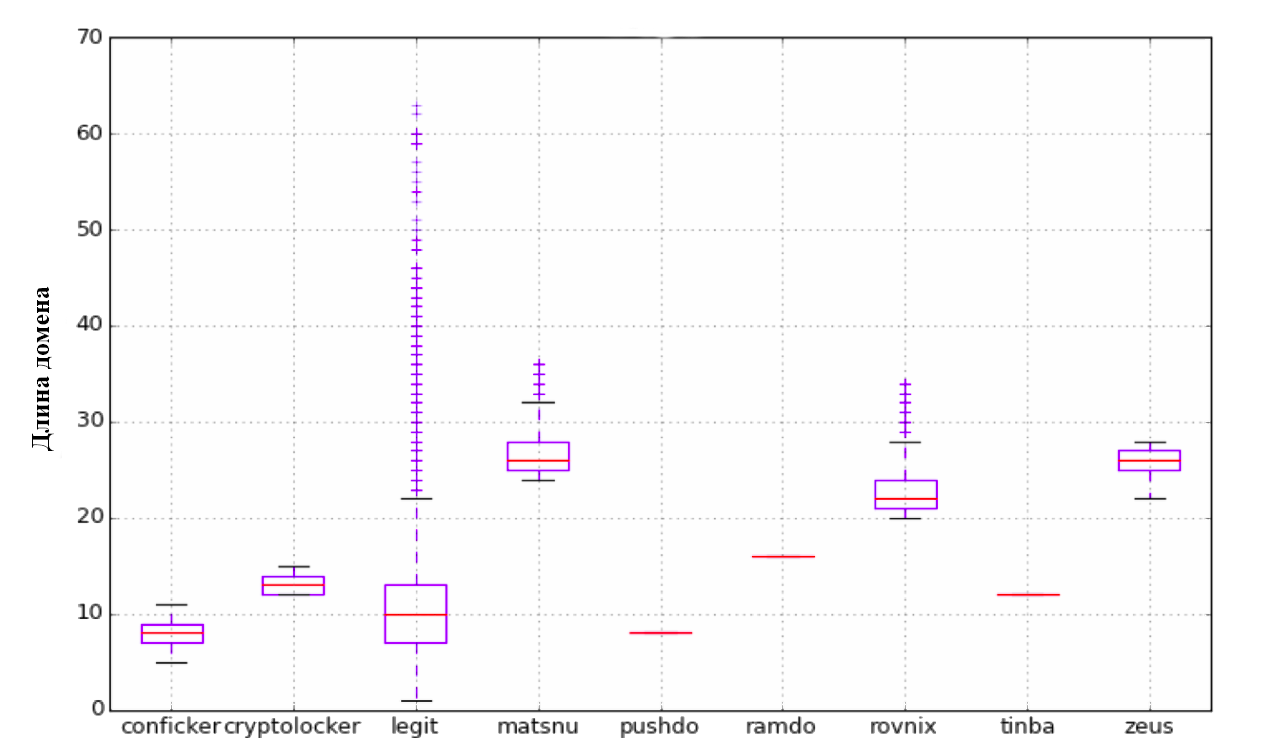
\includegraphics[width=0.5\linewidth]{images/linear_class/length.png}
        \right
        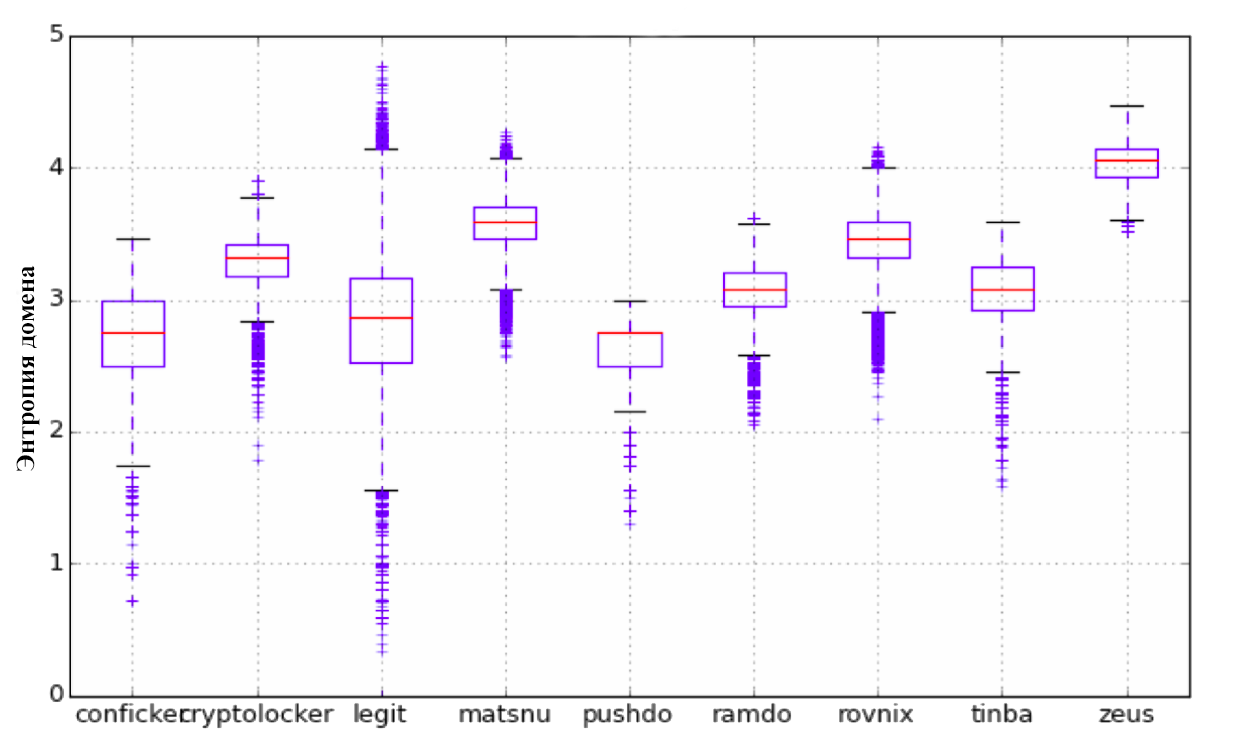
\includegraphics[width=0.5\linewidth]{images/linear_class/entropy.png} \label{length_entropy}
        \caption{Длина и энтропия доменных имен}
    \end{figure}
    \begin{figure}[H]
        \left
        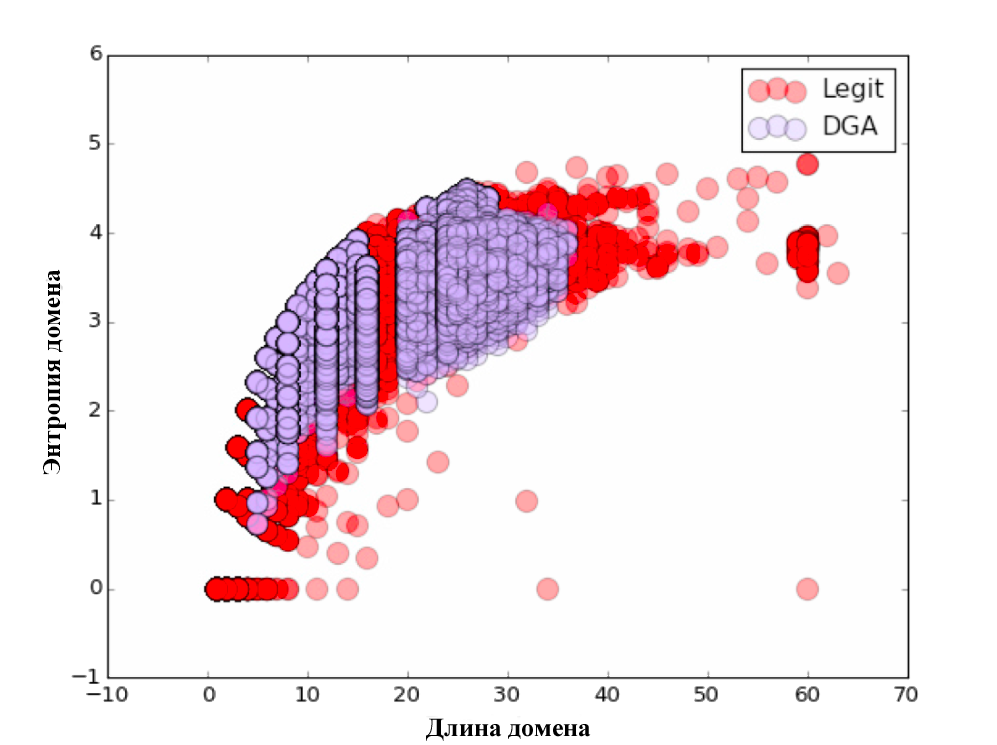
\includegraphics[width=0.5\linewidth]{images/linear_class/entropy2.png}
        \right
        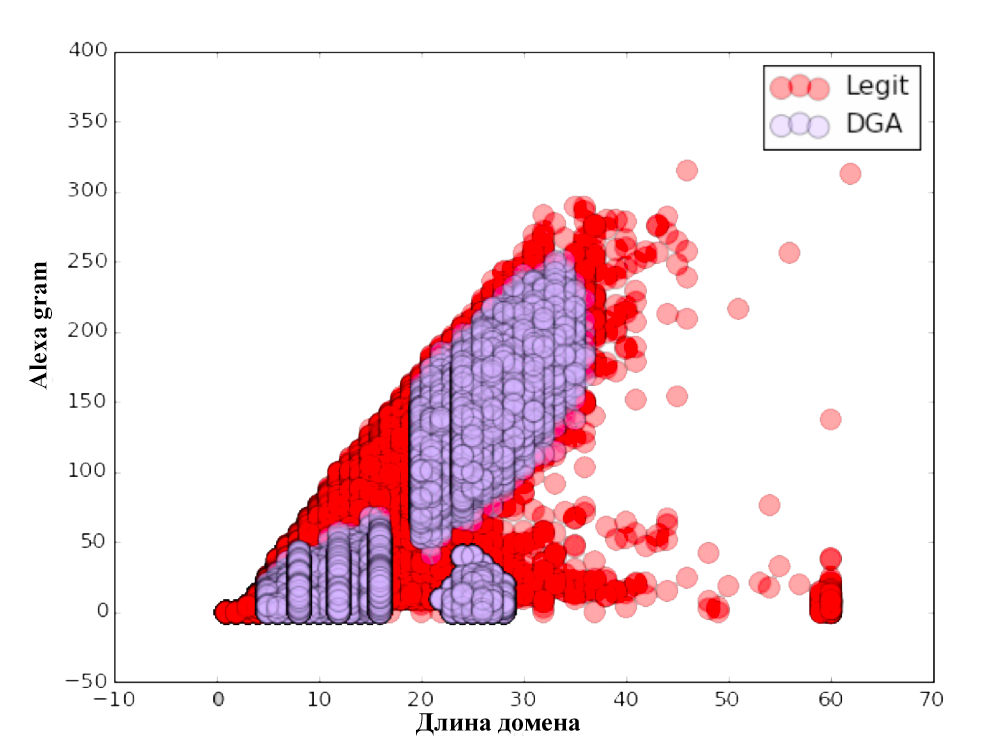
\includegraphics[width=0.5\linewidth]{images/linear_class/alexa_gramm.png}
        \caption{Зависимость энтропии и параметра alexa gram от длины доменного имени} \label{entropy_alexa}
    \end{figure}
    \begin{figure}[H]
        \left
        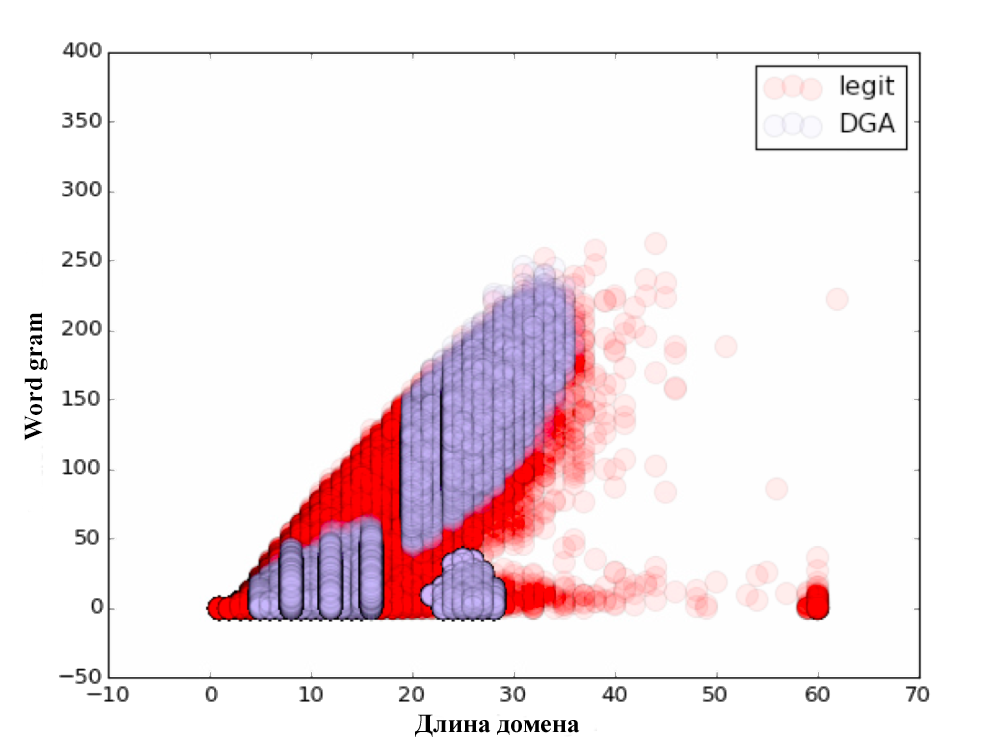
\includegraphics[width=0.5\linewidth]{images/linear_class/word_gramm.png}
        \right
        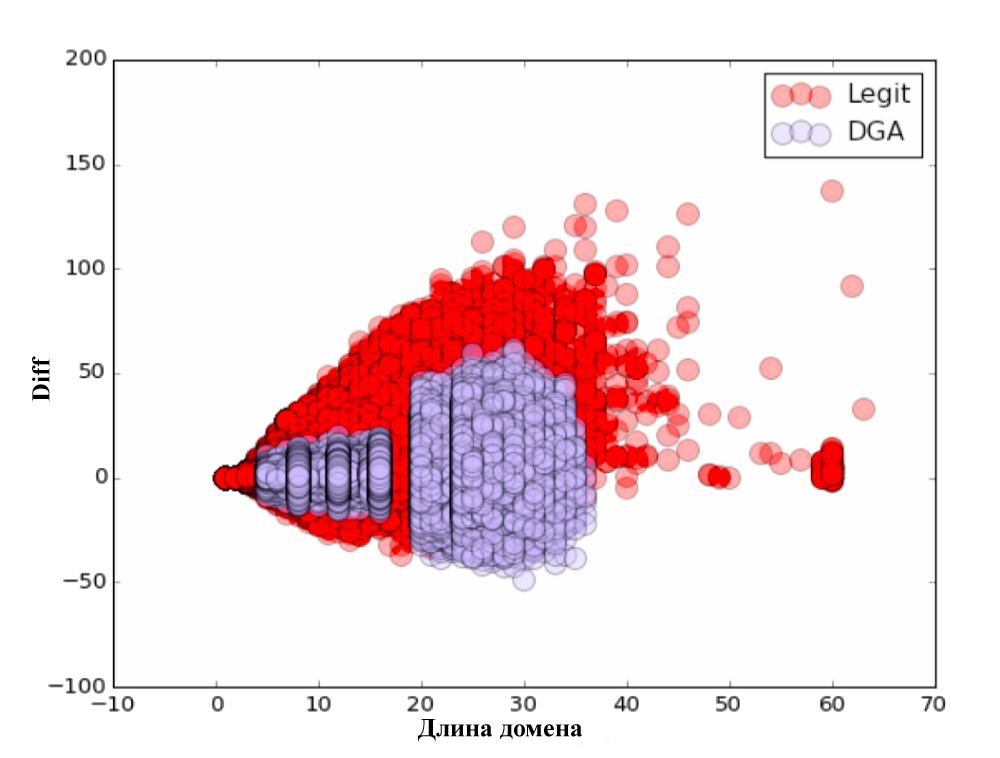
\includegraphics[width=0.5\linewidth]{images/linear_class/diff.png}
        \caption{Зависимость параметров word gram и diff от длины доменного имени} \label{word_gram_diff}
    \end{figure}
    Исходя из рис. 4.1 можно заметить, что вредоносные доменные имена не имеют длину менее 6 символов, что оправдывается высокой стоимостью таких доменных имен и повышенной вероятностью появления коллизий. Графики энтропии рис. 4.1 и рис. 4.2 доказывают, что, основываясь лишь на этом параметре, невозможно выделить вредоносные доменные имена в отдельный класс, так как множество значений энтропии вредоносных доменных имен является подмножеством множества значений энтропии легитимных доменных имен. А параметр diff на риc 4.3 был добавлен в модель после анализа параметров alexa gram и word gram. Вместе, эти параметры, позволяют выделить отдельные доменные имена в класс вредоносных.

    Процесс классификации проводился по принципу 80/20, т.е. обучение моделей проводилось на 80\% исходных данных, а тестирование на оставшихся 20\%. В качестве алгоритмов классификации использовались такие алгоритмы как:
    \begin{itemize}
    \item Logistic Regression;
    \item Random Forest;
    \item Naive Bayes;
    \item Extra Tree Forest;
    \item Voting Classification.
    \end{itemize}

    После тестировании и оценки качества классификации были получены следующие результаты:
    \begin{table}[ht]
    \centering
    \caption{Качество классификации}\label{}
    \begin{tabular}{@{}ccc@{}}
    \toprule
    Алгоритм              & Бинарная & Многоклассовая \\ \midrule
    Logistic Regression   & 86,7\%   & 78,8\%         \\
    Random Forest         & 95\%     & 89,3\%         \\
    Naive Bayes           & 75,2\%   & 75,6\%         \\
    Extra Tree Forest     & 94,6\%   & 88,9\%         \\
    Voting Classification & 94,7\%   & 90\%           \\ \bottomrule
    \end{tabular}
    \end{table}

    Автор провёл классификацию не только на вредоносные и легитимные домены, но и по принадлежности к определенному семейству DGA. В многоклассовой классификации наилучший результат показал алгоритм Voting Classification. Данный алгоритм реализован в библиотеке Scikit learn для языка программирования Python и представляет собой классификатор на основе результатов других статистических оценок. Однако, при распознавании вредоносных доменов лучше всего себя показал алгоритм Random Forest, заключающийся в использовании ансамбля решающих деревьев. Алгоритм сочетает в себе две основные идеи: метод Бэггинга Бреймана, и метод случайных подпространств, предложенный Tin Kam Ho.

    Для наглядности количественной оценки модели была построена матрица неточностей (confusion matrix), которая содержит правильно распознанные хорошие примеры (true positive), правильно распознанные плохие примеры (true negative) и ошибки в распознавании (false positive, false negative).
    \begin{table}[ht]
    \centering
    \caption{Матрица неточностей}\label{}
    \begin{tabular}{@{}cc@{}}
    \toprule
    Имя         & Точность \\ \midrule
    Legit/Legit & 95\%     \\
    Legit/DGA   & 5\%      \\
    DGA/Legit   & 4,3\%    \\
    DGA/DGA     & 95,7\%   \\ \bottomrule
    \end{tabular}
    \end{table}

    Наибольший интерес представляет показатель false positive, так как именно он, по мнению автора, определяет удобство использования данной модели в системе мониторинга инцидентов информационной безопасности. Изменяя различные параметры модели, в будущем можно добиться снижения этого показателя, не затрагивая качество отнесения доменнного имени к классу вредоносных.
    \subsection{Рекуррентные нейронные сети}\label{lstm_class_exp}
    В качестве эксперимента автор предлагает собственную модель, на основе модели рекуррентной нейронной сети, а именно модели Gated Recurrent Unit. Каждый домен в этом случае рассматривается как последовательность символов из фиксированного словаря, которая подаётся на вход рекуррентной нейронной сети. Обучение такой нейронной сети производится методом обратного распространения ошибки таким образом, чтобы максимизировать вероятность правильного выбора соответствующего класса. Для классификации, состояние последнего скрытого слоя передается в Softmax слой, выход которого мы можем интерпретировать как вероятности принадлежности домена к одному из классов. Полученная модель представлена на рис. \ref{baseline1}.
    \addimghere{images/lstm_class/baseline1}{0.6}{Модель 1}{baseline1}
    В ходе практического исследования данной модели автором найдено оптимальное значение скрытых нейронов. Данное значения равно 128 скрытым нейронам. %можно вставить 
    Кроме этого были протестированы различные алгоритмы стохастического градиентного спуска, такие как:
    \begin{itemize}
    \item SGD;
    \item Adadelta;
    \item Rmsprop;
    \item Adam.
    \end{itemize}
    В результате наилучший результат показал алгоритм Adam рис. \ref{sgd}, предложенный в статье [18]. Он является простым в реализации, вычислительно эффективным алгоритмом, имеет небольшие требования к памяти и хорошо подходит для задач, связанных с большим количеством данных и параметров.
    \addimghere{images/lstm_class/sgd.png}{0.6}{Алгоритмы стохастического градиентного спуска}{sgd}
    Далее, обучающая выборка была разбита на блоки по 100 доменных имен. В ходе обучения данной модели автором был получен следующий результат - рис. \ref{baseline1_res}.
    \addimghere{images/lstm_class/baseline1_res.png}{0.6}{Результат Модели 1}{baseline1_res}
    Однако были предприняты попытки по улучшению существующей модели. Так, одним из возможных методов повышения качества классификации является Модель 2, которая добавляет реверсивный проход по всей длине доменного имени. Это делается для того, чтобы иметь представление не только о прошлых входных значениях, но и о будущем контексте. Такая модель изображена на рис. \ref{baseline2}.
    \addimghere{images/lstm_class/baseline2}{0.6}{Модель 2}{baseline2}
    Как в Модели 1, так и в Модели 2 на вход в Softmax слой попадают состояние лишь последного скрытого слоя нейронной сети. Поэтому в качестве эксперимента автор предлает использовать механизма внимания, заключающийся в том, что все скрытые состояния нейронной сети складываются, умножаясь на определенный коэффициент, который также является обучаемым параметром нейронной сети:
    \begin{equation}\label{attention}
    H = a_{0}h_{0}+...+a_{t}h{t}
    \end{equation}
    \begin{equation}\label{coeff}
    \sum_{i=1}^{t} a_{i}=1
    \end{equation}
    В результате применения механизма внимания наша модель принимает вид рис. \ref{baseline3}.
    \addimghere{images/lstm_class/baseline3}{0.6}{Модель 3}{baseline3}
    Далее была разработана еще одна модель - Модель 4 рис. \ref{baseline4}. В отличии от Модели 3, данная модель применяет механизм внимания также и на прямой проход нейронной сети.
    \addimghere{images/lstm_class/baseline4}{0.6}{Модель 4}{baseline4}
    Для оценки сложности полученных моделей было подсчитано количество обучаемых параметров - таблица \ref{hard}. Она даёт представление о том, насколько отличаются по сложности каждая из предложенных моделей.
    \begin{table}[ht]
    \centering
    \caption{Сложность моделей}\label{hard}
    \begin{tabular}{@{}cc@{}}
    \toprule
    Модель         & Количество обучаемых параметров \\ \midrule
    Модель 1 & 67322     \\
    Модель 2 & 133114      \\
    Модель 3 & 249082    \\
    Модель 4 & 332282   \\ \bottomrule
    \end{tabular}
    \end{table}

    Используя алгоритм нелинейного снижения размерности и визуализации многомерных переменных t-SNE(t-distributed stochastic neighbor embedding, стохастическое вложение соседей с распределением Стьюдента) была произведена визуалиазация данных до и после обучения модели при задаче многоклассовой классификации рис. 4.10. Этот алгоритм обеспечивает эффективный метод визуализации сложных наборов данных. Он успешно обнаруживает скрытые структуры в данных, демонстрирует группы и компенсирует нелинейные отклонения по измерениям, сохраняя пропорции расстояний.
    
    \begin{figure}[H]
        \left
        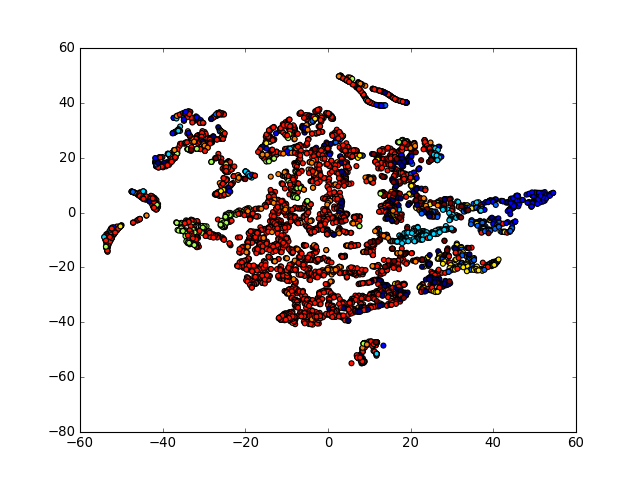
\includegraphics[width=0.5\linewidth]{images/lstm_class/not_train.png}
        \right
        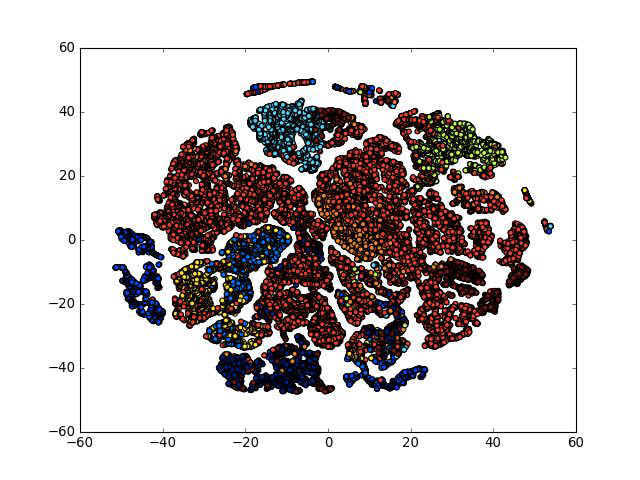
\includegraphics[width=0.5\linewidth]{images/lstm_class/train.png}
        \caption{Визуализация данных до и после обучения}\label{visual}
    \end{figure}
    Для оценки качества классификации все 4 модели были построены на 1 графике рис. 4.11:
    многоклассовая классификация - левый график, бинарная классификация - правый график.
    \begin{figure}[H]
        \left
        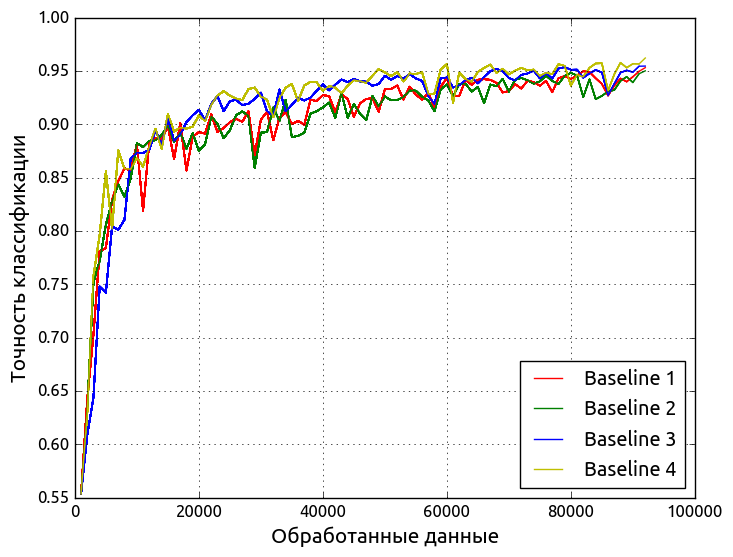
\includegraphics[width=0.5\linewidth]{images/lstm_class/all.png}
        \right
        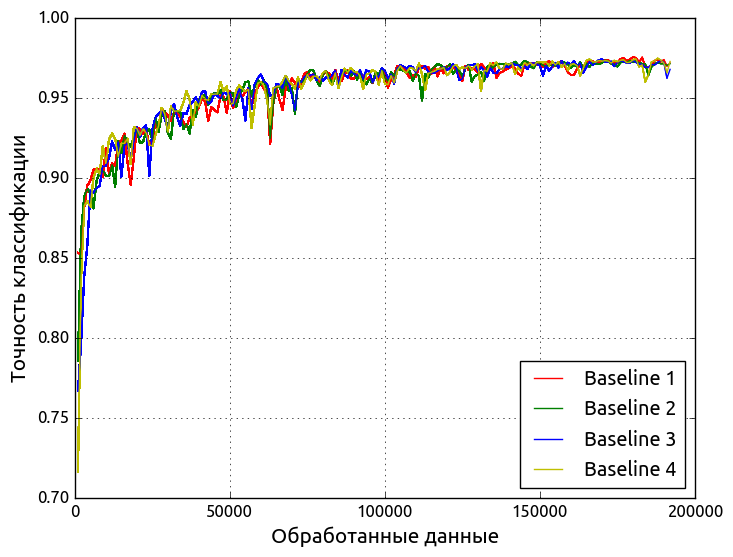
\includegraphics[width=0.5\linewidth]{images/lstm_class/2_class.png}
        \caption{Результаты многоклассовой и бинарной классификации}\label{length_entropy}
    \end{figure}
    В результате новая модель, построенная на основе рекуррентной нейронной сети повысила качество бинарной классификации до 97\%, а Модель 4 показала своё превосходство над другими моделями в многоклассовой классификации.
\clearpage